L’évolution des technologies et leurs usages ont fait exploser la quantité de données générées. Selon IBM, 2.5 milliard de gigabytes (GB) de données a été générée tout les jours de l'année 2012. De plus, cette quantité de données, double tout les deux ans. Cependant, seules 0,05\% de ces données sont analysées.\\

L’exploration ou la fouille de données (\og data mining \fg) consiste à en extraire des informations utiles, et ceci peut s’avérer très fructueux. La question principale qui se pose est de savoir comment utiliser intelligemment cette immense masse de données pour en tirer une plus-value ?\\
C’est le rôle des entreprises spécialisées dans l'exploitation de ces données.

\section{L'entreprise}
    La société Data Publica a été fondée en juillet 2011 par François Bancilhon et Christian Frisch, respectivement l'actuel directeur général et l'actuel directeur technique.

    \subsection{L'activité de Data Publica}
        Data Publica est un des précurseurs de l'open data en France. \textcolor{red}{Cette société , qui a bénéficiée d’investissements technologiques faits en 2010 dans le cadre d’un projet de R\&D, a été financée initialement par un groupe de business angels et le fonds d’amorçage \textbf{IT Translation}.}
        Data Publica est un start-up spécialisée dans les données entreprises, l'open data, le big data et la dataviz. C'est une société relativement jeune, axée R\&D. Son leitmotiv, alimenté par une équipe très dynamique et compétente, est la recherche constante du dépassement technique.

        \paragraph{}
            Historiquement, Data Publica ne faisait que de l'open-data. C'est-à-dire que la société se servait de données accessibles à tous (provenant d'institutions gouvernementales notamment) pour créer des jeux de données sur mesure pour des entreprises. Ainsi, la société s'est spécialisé dans l'identification des sources de données, leur extraction et leur transformation en données structurées.

        \paragraph{}
            Depuis quelques années, Data Publica se spécialise dans les données sur les entreprises française en dépit de son activité open-data qu'elle a progressivement mis de côté. Les services qu'elle propose ne sont plus tout-à-fait les mêmes. En effet, Data Publica réutilise les données open-data concernant les entreprises française dans son produit phare. Ce produit est lui même conçu pour les entreprises du B2B. Le produit est décrit en partie \ref{c_radar}.

        \paragraph{}
            Data Publica participe également à de nombreux projets de recherche français et européens tels que XDATA, Diachron ou Poqemon, en partenariat avec l'INRIA.

    \subsection{L'équipe de Data Publica}
        Data Publica emploie 14 personnes réparties en 2 équipes : une équipe commerciale (4 personnes) et une équipe technique (10 développeurs). Les deux équipes travaillent chacune dans son open-space. Pendant mon stage, j'ai été immergé au sein de l'équipe technique.

        \paragraph{L'équipe technique :}
            Elle est composé de 10 développeurs (ordonnés par ancienneté visible en figure \ref{fig:teamd_data_publica}) :
            \begin{itemize}
                \item Christian Frisch, directeur de l'équipe
                \item Thomas Dudouet, \textcolor{red}{Java / Back end développeur}
                \item Guillaume Lebourgeois, chef de produit C-Radar
                \item Samuel Charron, \textcolor{red}{Data scientist Python et mon maître de stage}
                \item Loïc Petit, \textcolor{red}{Java JBM}
                \item Clément Chastagnol, \textcolor{red}{data scientist Python et mon maître de stage}
                \item Clément Déon, \textcolor{red}{Front end développeur}
                \item Fabien Bréant, \textcolor{red}{Back end développeur}
                \item Jacques Belissent, \textcolor{red}{?}
                \item Vincent Ysmal, \textcolor{red}{Java / Back end développeur}
            \end{itemize}

        \begin{figure}[h!]
            \centering
            \begin{subfigure}[b]{0.2\textwidth}
                
\includegraphics[width=\textwidth]{images/christian-serieux.png}
                \caption{Christian F.}
            \end{subfigure}
            \begin{subfigure}[b]{0.2\textwidth}
                
\includegraphics[width=\textwidth]{images/thomas2-Copier-Copier.jpg}
                \caption{Thomas D.}
            \end{subfigure}
            \begin{subfigure}[b]{0.2\textwidth}
                
\includegraphics[width=\textwidth]{images/guillaume-serieux.png}
                \caption{Guillaume L.}
            \end{subfigure}
            \begin{subfigure}[b]{0.2\textwidth}
                
\includegraphics[width=\textwidth]{images/samuel-serieux.png}
                \caption{Samuel C.}
            \end{subfigure}
            \begin{subfigure}[b]{0.2\textwidth}
                
\includegraphics[width=\textwidth]{images/loic-serieux.png}
                \caption{Loïc P.}
            \end{subfigure}
            \begin{subfigure}[b]{0.2\textwidth}
                
\includegraphics[width=\textwidth]{images/clement-c-serieux.png}
                \caption{Clément C.}
            \end{subfigure}
            \begin{subfigure}[b]{0.2\textwidth}
                
\includegraphics[width=\textwidth]{images/clement-d-serieux.png}
                \caption{Clément D.}
            \end{subfigure}
            %\begin{subfigure}[b]{0.2\textwidth}
            %    
\includegraphics[width=\textwidth]{images/jacques.jpg}
            %            \caption{Jacques B.}
            %\end{subfigure}
            \begin{subfigure}[b]{0.2\textwidth}
                
\includegraphics[width=\textwidth]{images/vincent.jpg}
                \caption{Vincent Y.}
            \end{subfigure}
            \caption{L'équipe technique de Data Publica}
            \label{fig:teamd_data_publica}
        \end{figure}

\newpage

        \paragraph{L'équipe commerciale :}
            Elle est composé de 4 commerciaux (ordonnés par ancienneté) :
            \begin{itemize}
                \item François Bancilhon, directeur général
                \item Benjamin Gans, Responsable Communication et Marketing
                \item Emmanuel Jouanne, Business Development Manager
                \item Philippe Spenato, Ingénieur d'affaire
                \item Justine Pourrat, Responsable Communication et marketing
            \end{itemize}

        \begin{figure}[h!]
            \centering
            \begin{subfigure}[b]{0.2\textwidth}
                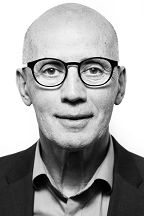
\includegraphics[width=\textwidth]{images/francois-serieux.png}
                \caption{François B.}
            \end{subfigure}
            \begin{subfigure}[b]{0.2\textwidth}
                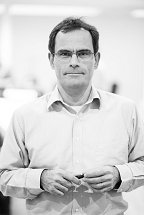
\includegraphics[width=\textwidth]{images/philippe-1-serieux.png}
                \caption{Philippe S.}
            \end{subfigure}
            \begin{subfigure}[b]{0.2\textwidth}
                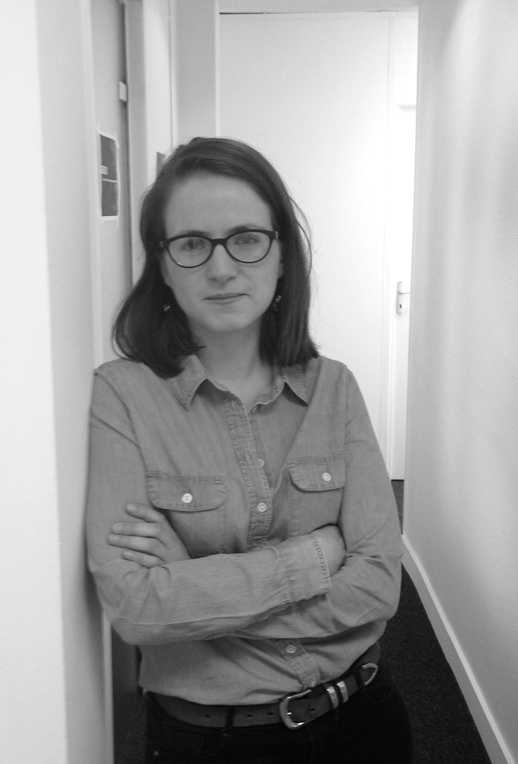
\includegraphics[width=\textwidth]{images/Justine-serieuse-crop.jpg}
                \caption{Justine P.}
            \end{subfigure}
            \caption{L'équipe commerciale de Data Publica}
            \label{fig:teamc_data_publica}
        \end{figure}

\section{C-Radar}\label{c_radar}
    \subsection{Présentation commerciale de C-Radar}
        Son produit est un moteur de recherche B2B (Business to Business). Celui-ci a pour objectif de permettre aux services ventes et marketing des entreprises B2B de vendre plus et mieux.\\
        Ce moteur de recherche, appelé C-Radar, est un produit de vente prédictive construit sur une base de référence des entreprises françaises. Il regroupe beaucoup d'informations sur les entreprises françaises, dont notamment leurs informations administratives, financières et toutes celles qui découlent de leur communication sur les réseaux sociaux et le web.\\

        C-Radar est un concentré de technologies du big data. En effet, il utilise diverses technologies comme le crawling, le scraping ou encore le machine learning. Ceci afin d'offrir à l'utilisateur diverses fonctionnalités : moteur de recherche d'entreprises, fiche d'activité d'entreprises avec contacts commerciaux, détection de nouveaux prospects, scoring de prospects existants, segmentation automatique d'entreprises, identification de marché, etc.

    \subsection{Présentation technique de C-Radar}
        \subsubsection{Les technologies utilisées par C-Radar}
            Pour répondre aux problématiques auxquelles Data Publica se confronte, la société a acquis 4 expertises majeures :
            \begin{itemize}
                \item Le web crawling / web scraping : la récupération des données ;
                \item Le data mining / text mining : l'analyse, l’extraction et l’enrichissement des données;
                \item Le machine learning : l'apprentissage automatique à partir de données structurées ;
                \item La dataviz : la visualisation des données.
            \end{itemize}

            \paragraph{Le crawling :}
                Le crawling est l’action réalisée par un programme informatique, appelé le web crawler, qui va de site en site afin d’en extraire automatiquement toute l’information qui est présente sur les différentes pages. Cette technique est utilisée notamment pour l’extraction de données non structurées: la structure du site n’est pas connue à l’avance, l’extraction des données se fait directement sur le contenu (c’est à dire le code HTML) de la page crawlée. Ce processus est \og brutal \fg.

            \paragraph{Le scraping :}
                Le scraping est l’action réalisée par un programme informatique pour extraire des unités d’information structurées d’un site web. Contrairement au crawling, il est question d’extraire des données précises, et pas la totalité des données disponibles sur le site. Le site “scrappé” et sa structure doivent donc être connus et analysés à l’avance afin d’adapter le scraper au site. Ce processus est \og intelligent \fg.

            \color{red}

            \paragraph{Le data mining / text mining :}
                Une fois des sites web crawlés et scrapés, ou que des flux (RSS ou réseaux sociaux) aient été captés, on peut commencer à analyser le contenu récupéré à la recherche d'informations sous forme de patterns particuliers, par exemple. On analyse afin de normaliser des problèmes d'encodages, de structures de date, de numéros de téléphone, etc.\\
                Globalement, cette phase consiste à regarder les données \og dans le fonds des yeux \fg \autocite{steph_canu} afin de voir leurs fonds mais aussi leurs formes.

            \paragraph{Le machine learning :}
                Quand les données sont correctement formatées et normalisées, on peut construire des applications capable d'apprendre automatiquement de ces données, de les classifier. Ainsi quand on aura une nouvelle donnée l'application sera capable de prédire sa classe d'après ses caractéristiques.\\
                L'idée derrière le machine learning est de pouvoir extraire automatiquement des informations d'une nouvelle donnée et ainsi prédire une classe de donnée.

            \paragraph{La dataviz :}
                C'est la dernière étape. Elle présente les données de manière visuelle et interprétable. Ainsi, on peut comprendre plus facilement et rapidement les informations extraites des données.


        \subsubsection{L'architecture technique de C-Radar}
            L'architecture de C-Radar peut être divisée en plusieurs parties (visible en figure \ref{fig:archi}) :
            \begin{itemize}
                \item Différentes bases de données pour différents stockages (une base de données Mongo, une base de données Cassandra et une base de données PostGreSQL) ;
                \item Un moteur de recherche sémantique (Elastic Search) ;
                \item Un gestionnaire de queue (RabbitMQ) ;
                \item Différents plugins Python s'interfaçant avec le gestionnaire de queue RabbitMQ ;
                \item Un gestionnaire de flux entre les différents composants précédents, le Workflow ;
                \item Une application Java s'interfaçant avec Elastic Search et les bases de données Mongo et PostGreSQL.
            \end{itemize}

            \paragraph{Le JBM ou Java Base Manager :}
                Le JBM est le projet Java qui rassemble le Workflow et l'application \href{app.c-radar.com}{app.c-radar.com}. Ce projet a été conçu et construit au dessus de Spring. Spring est un framework Java permettant de créer des applications web. Il prend en charge énormément de chose dont notamment le modèle MVC, la sécurité de l'application, l'interface avec les gestionnaire de queue, etc. (Pour plus d'information, voir \href{http://spring.io/}{http://spring.io/}).

            \paragraph{Le Workflow :}
                Le Workflow est le gestionnaire de flux permettant de lancer les différents processus de récupération et d'analyses des données. Il gère tout ce qui est \og computing \fg. Par exemple, c'est lui qui lance RabbitMQ qui lui même lance l'exécution des plugins Python gérant le processus de crawling de sites web, par exemple. Une fois les sites webs crawlés, le Workflow va les stocker dans Cassandra. Il gère tout ce qui est exécution des plugins Python (crawling et scraping du web, capture et catégorisation des signaux, etc), stockage des données produites à l'issue de ces exécutions et indexation dans Elastic Search.\\
                Pour résumer, il prépare les données que l'application va se charger de présenter à l'utilisateur.

            \paragraph{L'application \href{app.c-radar.com}{app.c-radar.com} :}
                L'application, \og présente \fg les données aux utilisateurs. Elle fait le reporting des données produites par le Workflow. Elle permet de rechercher des entreprises, de voir leur répartitions géographiques, de créer des listes d'entreprises, etc. C'est l'application visible et utilisée par l'utilisateur.

            \paragraph{Les bases de données :}
                Les bases de données stockent différentes données. La base Mongo stocke les données liées aux entreprises et les signaux, par exemple.

            \paragraph{Les plugins Python :}
                Enfin, les plugins Python sont des applications Python connectées à d'autres composants, afin d'exécuter une tâche sur des données. Ces données sont reçues des autres composants et le plugin leur retourne les résultats de sa tâche.

            \color{black}


            \begin{figure}[h!]
                \centering
                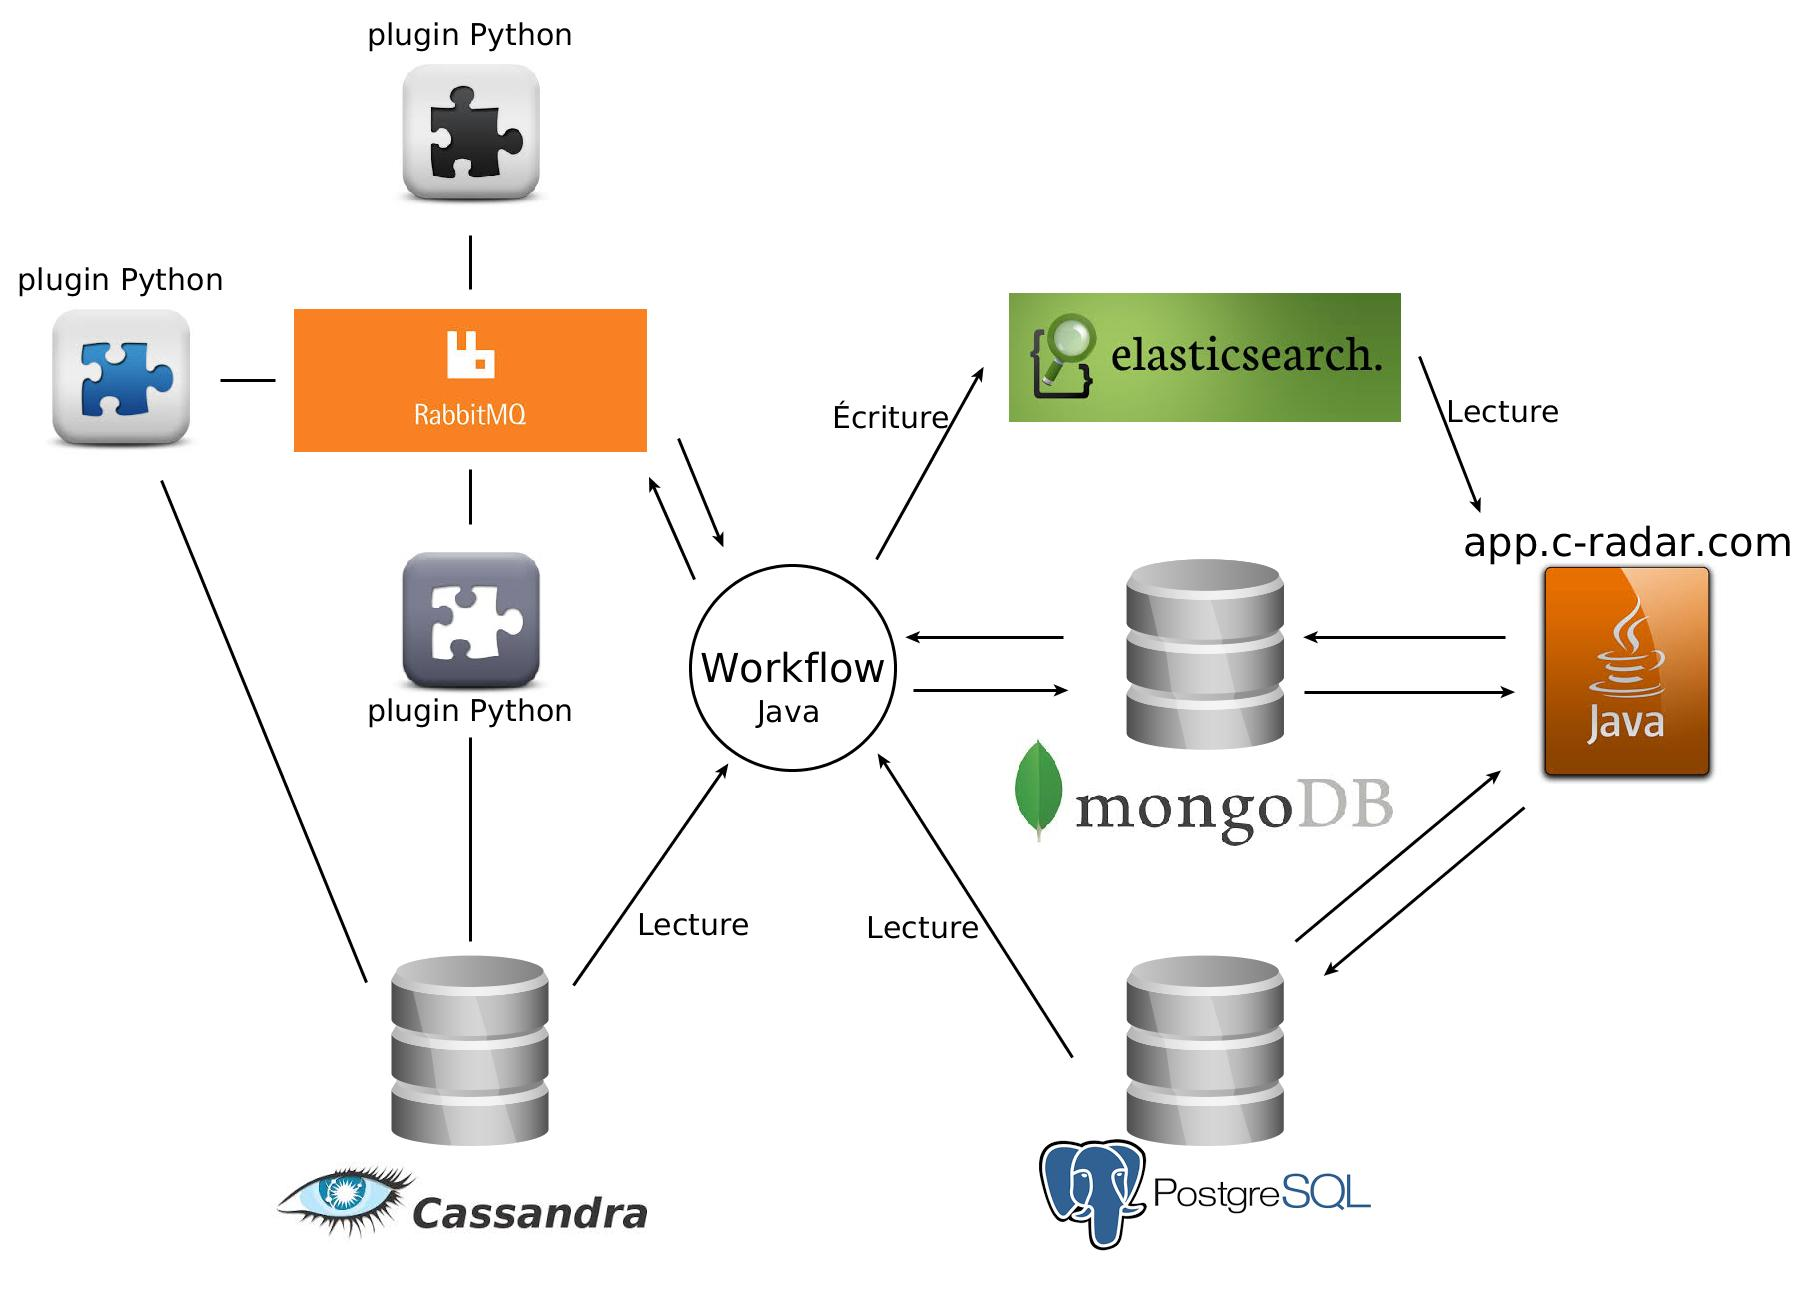
\includegraphics[width=\textwidth]{images/archi.jpg}
                \caption{L'architecture générale de C-Radar}
                \label{fig:archi}
            \end{figure}